\chapter{ANALISIS SOLUSI DAN ARSITEKTUR SISTEM}

Bab ini menjelaskan mengenai arsitektur lingkungan simulasi sebagai tempat uji coba, detail analisis masalah, desain arsitektur solusi, dan desain algoritma estimasi yang dapat digunakan.

\section{Arsitektur Lingkungan Simulasi}

\begin{figure}[h]
    \centering
    \medskip
    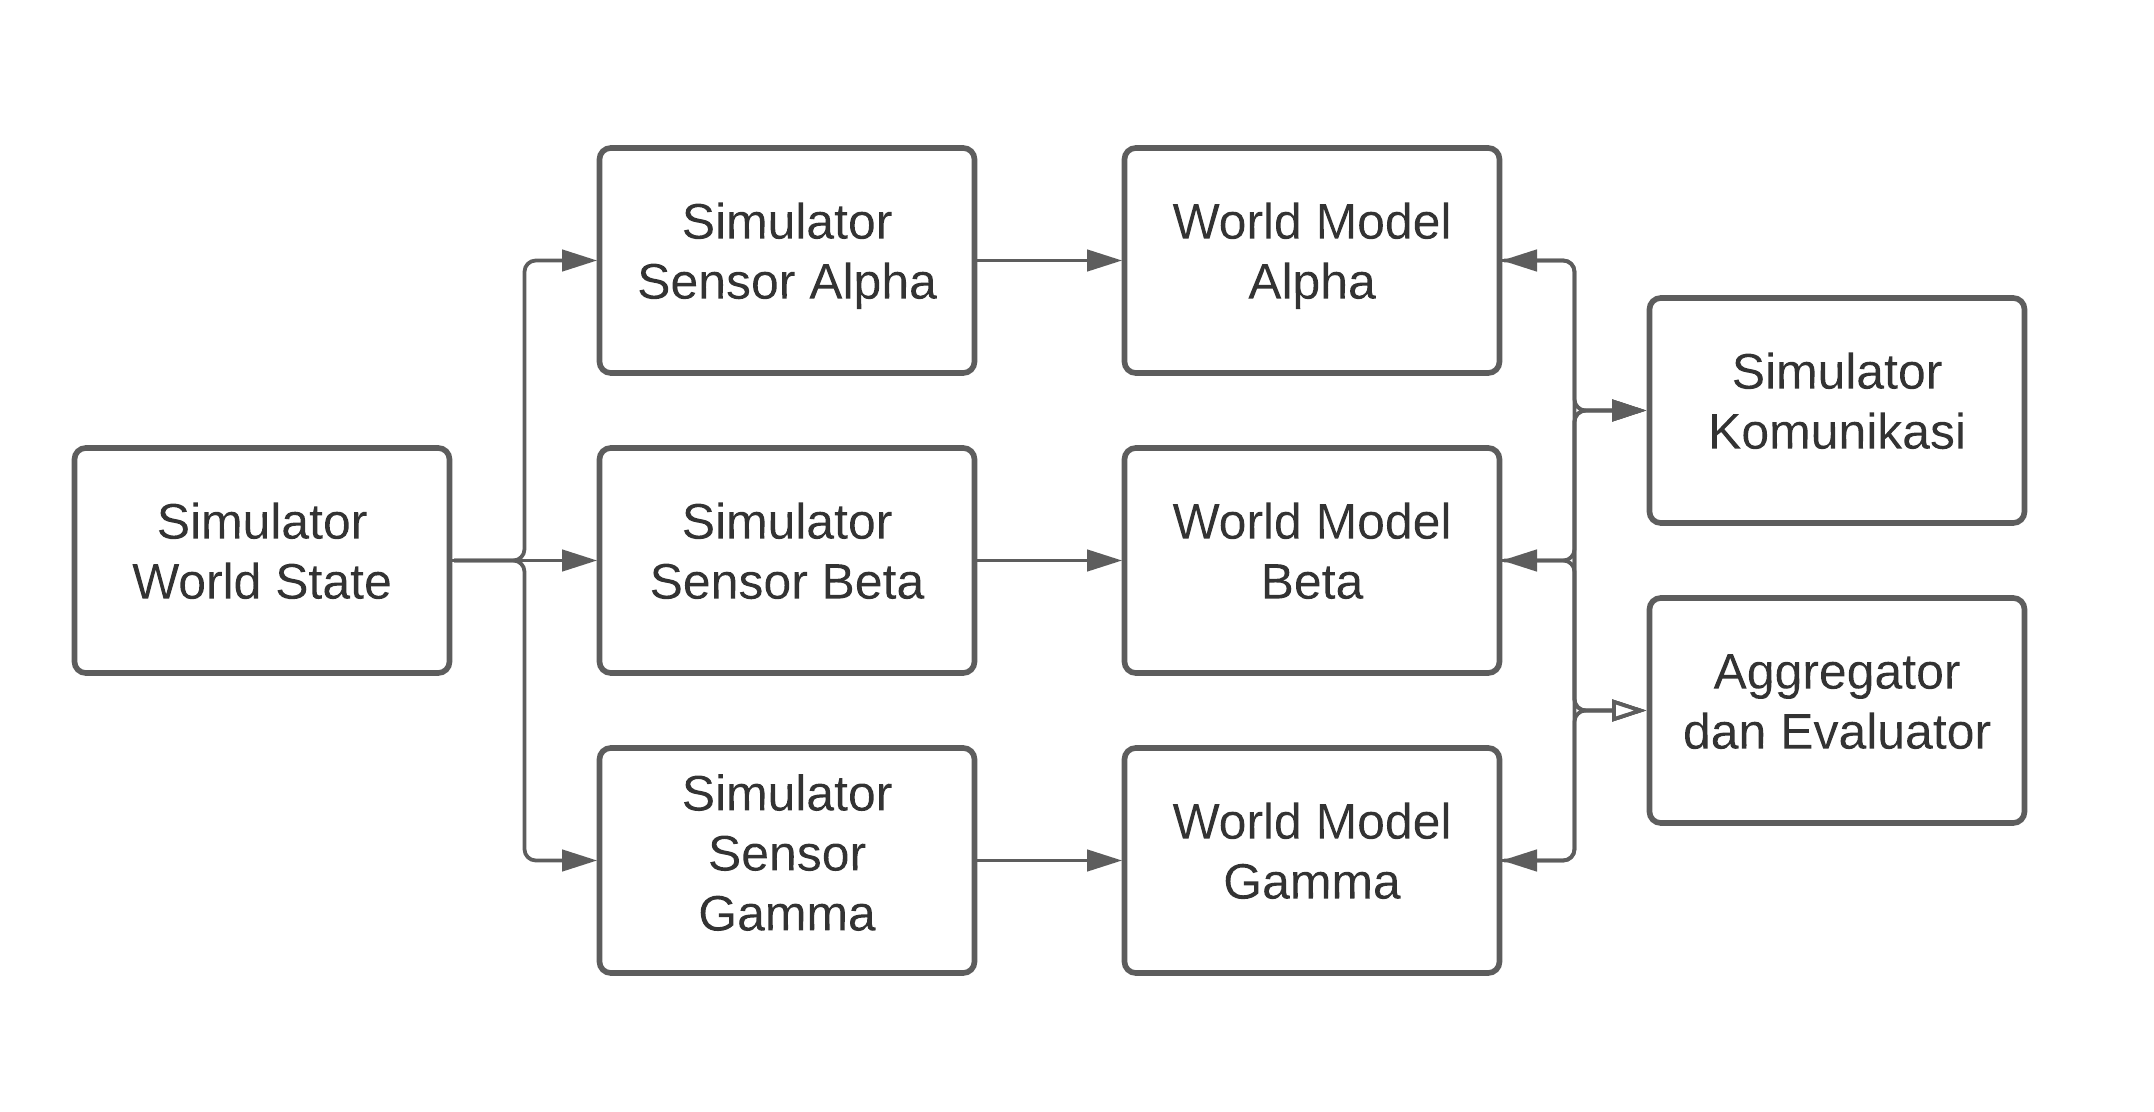
\includegraphics[width=0.8\textwidth]{resources/simulation-structure.png}
    \caption{Struktur modul simulasi}
    \label{fig:simulation-structure}
    \bigskip
\end{figure}

Lingkungan simulasi dikembangan dalam \textit{framework} ROS, dimana arsitektur lingkungan simulasi digambarkan di \ref{fig:simulation-structure} dimana masing-masing \textit{node} berjalan dengan periode komputasi $30$ ms yang didasari pada periode ketersediaan data sensor di keadaan nyata. Selain \textit{node} \textit{world model} yang bertugas untuk menampung algoritma estimasi \textit{world state}, terdapat beberapa \textit{node} simulator yang bertujuan untuk membangkitkan data pengujian untuk menganalisis akurasi algoritma estimasi.

\subsection{Simulator \textit{World State}}

\begin{figure}[h]
    \centering
    \medskip
    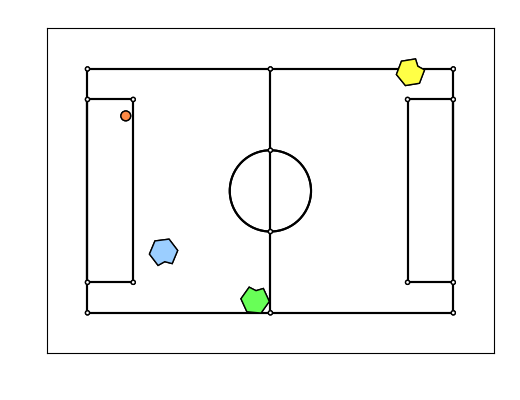
\includegraphics[width=0.8\textwidth]{resources/true-world-state.png}
    \caption{Keadaan \textit{world state} sesungguhnya}
    \label{fig:true-world-state}
    \bigskip
\end{figure}

Modul simulator \textit{world state} seperti pada \ref{fig:true-world-state} bertujuan untuk membangkitkan nilai \textit{world state} uji coba yang sebenarnya, yang mencakup pergerakan dari masing-masing robot tim dan bola. Simulasi dilakukan di lapangan $9 \times 6$ meter kuadrat sesuai spesifikasi pertandingan regional Kontes Robot Indonesia cabang sepak bola beroda tahun 2019. Terdapat dinding dengan jarak satu meter di sekitar lapangan untuk mencegah robot dan terutama bola untuk keluar dari lapangan. Tiga robot tim yang disimulasikan, bernama alpha, beta, dan gamma, digerakan oleh suatu perencana gerakan sementara yang sekali-kali membangkitkan target \textit{pose} yang harus dituju oleh robot terkait. Masing-masing robot lalu mendekati target \textit{pose} masing-masing dengan gerakan lurus sekaligus dengan rotasi dengan kecepatan maksimum $2$ meter per detik dan akselerasi maksimum $1.5$ meter per detik kuadrat. Pergerakan bola dibangkitkan dengan terus meng\textit{update} kecepatan bola setiap periode komputasi dengan perubahan kecepatan di sumbu x dan y mengikuti distribusi normal dengan variansi sebesar $0.16$ meter per detik dikuadratkan dikali periode komputasi, dan kecepatan maksimal $2$ meter per detik. Simulator \textit{world state} juga mengecek apakah terjadi tabrakan antar robot, bola, ataupun dinding, dimana bola akan memantul sedangkan robot akan berhenti dan menghasilkan target \textit{pose} baru untuk keluar dari tabrakan.

\subsection{Simulator Sensor}

\begin{figure}[h]
    \centering
    \medskip
    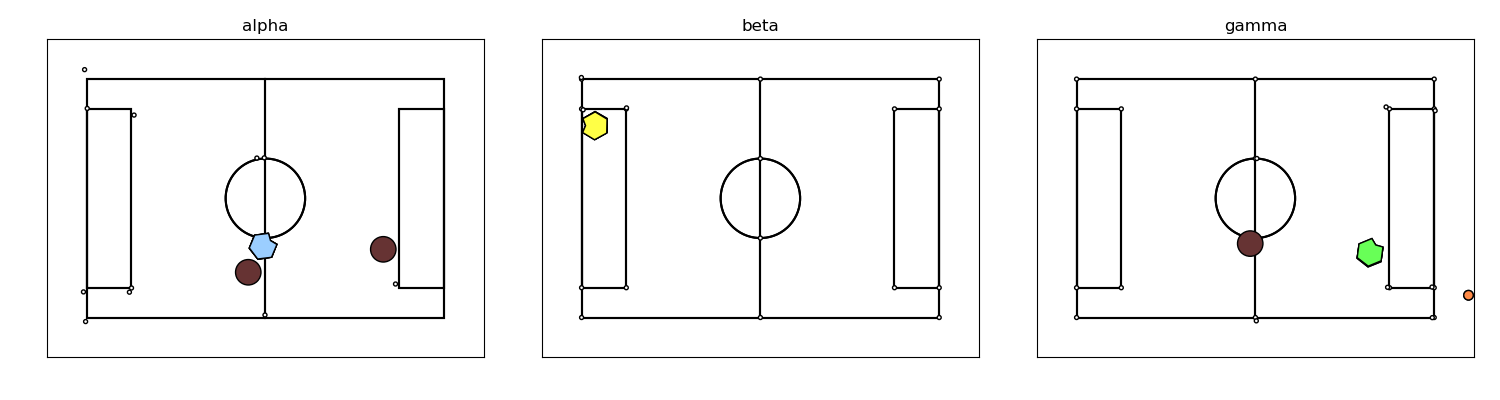
\includegraphics[width=\textwidth]{resources/allies-sensor.png}
    \caption{Bacaan sensor masing-masing robot}
    \label{fig:allies-sensor}
    \bigskip
\end{figure}

Terdapat tiga \textit{node} simulator sensor untuk masing-masing robot yang mengikuti pesan \textit{world state} dari \textit{node} simulator \textit{world state} dan menghitung hasil bacaan sensor dari robot tersebut, yang mencakup simulasi bacaan odometri berupa perpindahan \textit{pose} dari robot terhadap \textit{pose} di periode komputasi sebelumnya; simulasi bacaan kompas berupa orientasi absolut dari robot; dan simulasi persepsi \textit{vision} dari kamera yang mencakup posisi relatif dari \textit{landmark}, bola apabila terlihat, dan teman yang terlihat. \textit{Landmark} merupakan $16$ titik-titik statis yang tersebar di sekitar lapangan yang dapat dilihat oleh robot untuk membantu proses lokalisasi dari robot tersebut. Persepsi \textit{vision} terbatas dalam suatu rentang penglihatan robot sebesar radius maksimal $4$ meter yang juga terpengaruh oleh oklusi terhalangnya suatu objek oleh objek lain, seperti robot teman menghalangi persepsi bola atau \textit{landmark} dibelakangnya, atau suatu peluang kecil dimana suatu objek yang harusnya terlihat gagal dideteksi oleh \textit{vision} seperti pada \ref{fig:allies-sensor}. \textit{Vision} tidak dapat membedakan antara satu \textit{landmark} dengan \textit{landmark} lainnya ataupun satu teman dengan lainnya.

Masing-masing bacaan ditambahkan \textit{error} dengan variansi yang proporsional terhadap bacaan sesungguhnya. Bacaan odometri memiliki \textit{error} dengan variansi sebesar jarak perpindahan sebenarnya dikali sekitar $0,02$. Sedangkan bacaan \textit{vision} memiliki \textit{error} dengan variansi sebesar jarak objek sebenarnya dikali $0,0036$ untuk \textit{error} sejajar dengan arah objek dan $0,0009$ untuk \textit{error} tegak lurus arah objek.

\subsection{Simulator Komunikasi}

\begin{figure}[h]
    \centering
    \medskip
    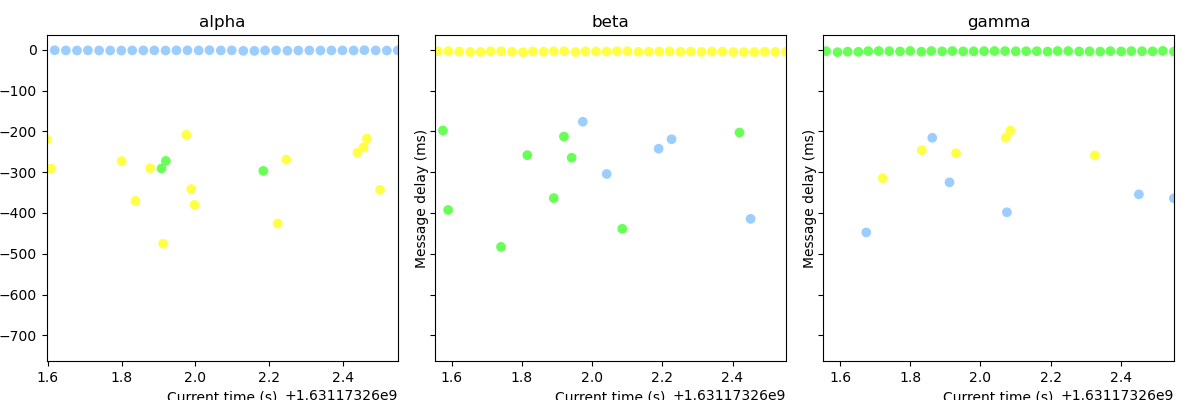
\includegraphics[width=\textwidth]{resources/allies-comm.png}
    \caption{Latensi komunikasi}
    \label{fig:allies-comm}
    \bigskip
\end{figure}

\textit{Node} \textit{world model} dapat menyiarkan pesan ke temannya, yang akan diterima oleh \textit{node} simulator komunikasi dan disiarkan balik ke semua temannya setelah suatu latensi komunikasi dan peluang hilangnya pesan. Simulator komunikasi dimodelkan dengan hidden Markov model dengan dua \textit{state}, yang menandakan kondisi jaringan baik dengan latensi komunikasi berdistribusi \textit{shifted gamma} dengan rata-rata $35$ ms, minimum $20$ ms, standar deviasi $10$ ms, dan kemungkinan hilangnya pesan sebesar $5\%$; dan kondisi jaringan buruk dengan latensi dengan rata-rata $300$ ms, minimum $150$ ms, standar deviasi $100$ ms, dan kemungkinan hilangnya pesan sebesar $65\%$.

\subsection{Aggregator dan Evaluator}

\begin{figure}[h]
    \centering
    \medskip
    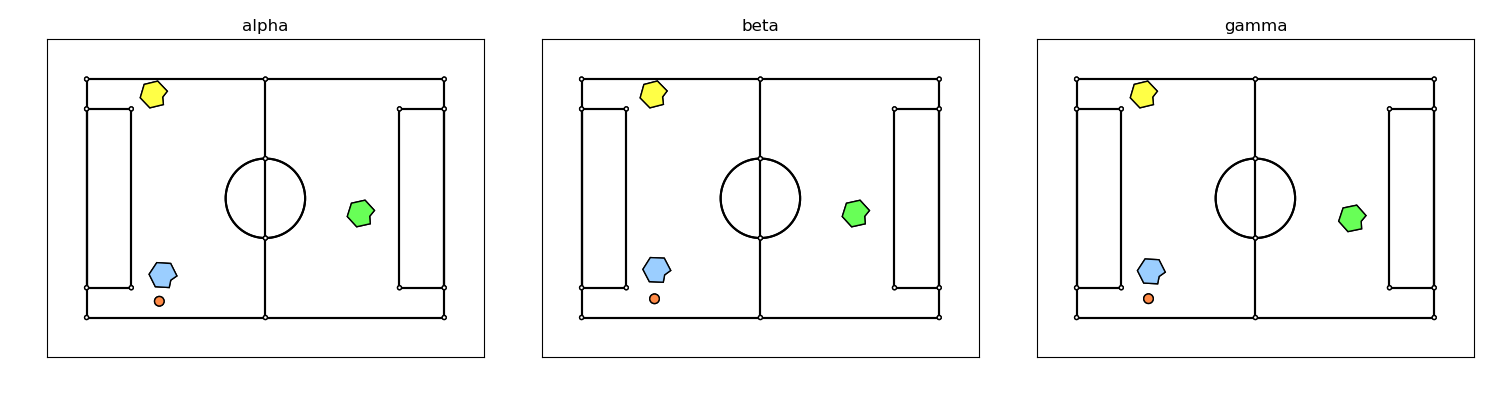
\includegraphics[width=\textwidth]{resources/allies-world-model.png}
    \caption{Estimasi \textit{world state} masing-masing robot}
    \label{fig:allies-world-model}
    \bigskip
\end{figure}

\textit{Node-node} aggregator dan evaluator mengikuti hasil estimasi dari \textit{world model} yang ada dan nilai sebenarnya dari \textit{world state} untuk melakukan evaluasi kinerja algoritma dan hal lain seperti visualisasi seperti pada \ref{fig:allies-world-model}. Evaluasi performa dari suatu algoritma diambil dari metrik \textit{error} berupa jarak hasil estimasi dan keadaan sebenarnya dari masing-masing objek dimana nilai $I/M$ dari robot bernilai $0.4$.

\section{Analisis Studi Terdahulu}

Dari studi yang sudah diteliti, didapat bahwa walaupun sudah cukup banyak studi yang membahas mengenai algoritma estimasi \textit{world model} yang melacak posisi robot maupun bola di kontes robot sepak bola, hampir semua studi tersebut mengasumsikan bahwa komunikasi antar robot memiliki latensi yang dapat diabaikan. Studi yang melakukan pengujian pada kasus kegagalan komunikasi berjumlah sedikit dan juga hanya menguji kasus kegagalan komunikasi total pada suatu robot. Banyak algoritma yang dibahas dari studi sebelumnya tidak dapat bekerja secara efektif dalam keadaan latensi komunikasi yang signifikan, seperti teknik merata-ratakan data, menggabungkan distribusi Gaussian data, maupun melakukan minimasi \textit{error} terhadap sistem. Algoritma \citet{ahmad2017} dibahas sebagai algoritma yang bersifat \textit{online} yang tidak membutuhkan terkumpulnya informasi dari robot-robot lainnya sebelum suatu robot dapat mulai melakukan kalkulasi estimasi, tetapi studi tersebut tetap tidak menangani integrasi data yang terlambat dan di luar urutan.

Secara umum, di luar konteks kontes robot sepak bola beroda, walau terdapat banyak studi yang membahas penggabungan data dari banyak sensor dengan latensi dan keterlambatan, masih sedikit studi yang membahas penggabungan data pengukuran sensor dengan latensi pada sistem komputasi terdesentralisasi, dimana dapat dilakukan suatu pemrosesan data terlebih dahulu sebelum dilakukannya komunikasi, dan hasil pemrosesan terjadi di masing-masing agen dengan hasil yang tidak harus sama.

\section{Arsitektur Umum Solusi}

Dalam pemrograman \textit{node} \textit{world model} dalam ROS yang berjalan berdasarkan fungsi \textit{callback} yang dipanggil setiap \textit{node} menerima pesan atau fungsi yang dijadwalkan untuk dipanggil dalam suatu frekuensi, terdapat tiga fungsi yang harus diimplementasi, yaitu fungsi saat \textit{node} mendapat data sensor, saat \textit{node} mendapat data dari teman, dan untuk setiap periode komputasi ($30$ ms).

Pertama, selain menyimpan estimasi gerakan untuk robot tim dan bola, \textit{node} juga sebaiknya menyimpan \textit{timestamp} dari data terakhir dari masing-masing objek yang diestimasi. Hal ini dikarenakan algoritma penapis yang digunakan pada dasarnya memproses data secara sekuensial terhadap waktu untuk menghasilkan estimasi pada waktu data yang terakhir. Oleh karena itu, estimasi yang disimpan oleh \textit{node} juga merupakan estimasi pada \textit{timestamp} dari data terakhir objek tersebut. Maka agar hasil estimasi yang dihasilkan \textit{world model} faktual dengan waktu sekarang yang sesungguhnya, dilakukan penyesuaian dengan memprediksi gerakan objek pada waktu sekarang. Prediksi dilakukan dengan mengasumsikan kecepatan atau \textit{twist} dari objek bernilai konstan dan meng\textit{update} posisi atau \textit{pose} dari objek tersebut berdasarkan selisih waktu antara waktu sekarang dan \textit{timestamp} masing-masing objek.

Karena walaupun dalam keadaan kegagalan komunikasi, robot masih harus menjalankan fungsionalitas dasarnya seperti navigasi setiap saat, maka masing-masing robot tim sebaiknya tetap memproses data sensornya masing-masing untuk mendapatkan informasi seperti gerakan robot sendiri, bola, dan mungkin objek di sekitarnya. Algoritma sebaiknya dapat berjalan secara \textit{online} tanpa harus menunggu informasi dari robot lain terlebih dahulu sebelum dapat berjalan dengan akurat.

Data sensor robot sendiri yang mengandung informasi odometri, orientasi kompas, dan persepsi \textit{landmark} merupakan sumber informasi yang paling dapat diandalkan untuk menentukan \textit{pose} atau gerakan secara umum dari robot sendiri. Oleh karena itu, dalam fungsi \textit{callback} sensor sebaiknya melakukan estimasi gerakan robot sendiri atau lokalisasi. Selain itu, data persepsi \textit{bola} yang merupakan satu-satunya sumber informasi mengenai gerakan bola juga sebaiknya diproses dan diestimasi apabila robot tersebut melihat bola. Hasil estimasi gerakan robot sendiri dan bola ini apabila terlihat disebarkan ke semua teman untuk dipakai ke dalam hasil estimasi dari \textit{node} \textit{world model} semua robot dalam tim. Pesan yang disebarkan tersebut mengandung \textit{timestamp} dari waktu sensor robot agar teman yang menerima pesan tersebut dapat mengetahui kapan data terkandung dilihat dan memutuskan bagaimana cara untuk mengintegrasi data tersebut.

Selain menyimpan informasi gerakan dari robot teman, apabila teman tersebut menyebarkan informasi gerakan bola, informasi tersebut juga sebaiknya diintegrasikan ke dalam hasil estimasi robot sendiri, terutama apabila \textit{timestamp} dari data tersebut lebih baru dari \textit{timestamp} data bola terakhir yang dimiliki robot sendiri. Ini terjadi saat sensor \textit{vision} yang dimiliki robot sendiri tidak melihat bola dalam radiusnya atau karena terjadi oklusi untuk cukup lama sehingga informasi dari teman yang melihat lebih baru dari terakhir robot sendiri dapat melihat bola. Selain itu, informasi dengan \textit{timestamp} lebih lama dari informasi yang sudah dimiliki seperti informasi gerakan teman dapat diabaikan karena informasi yang lebih baru sudah mencakup dan kemungkinan lebih akurat dari informasi tersebut.

\begin{figure}[h]
    \centering
    \medskip
    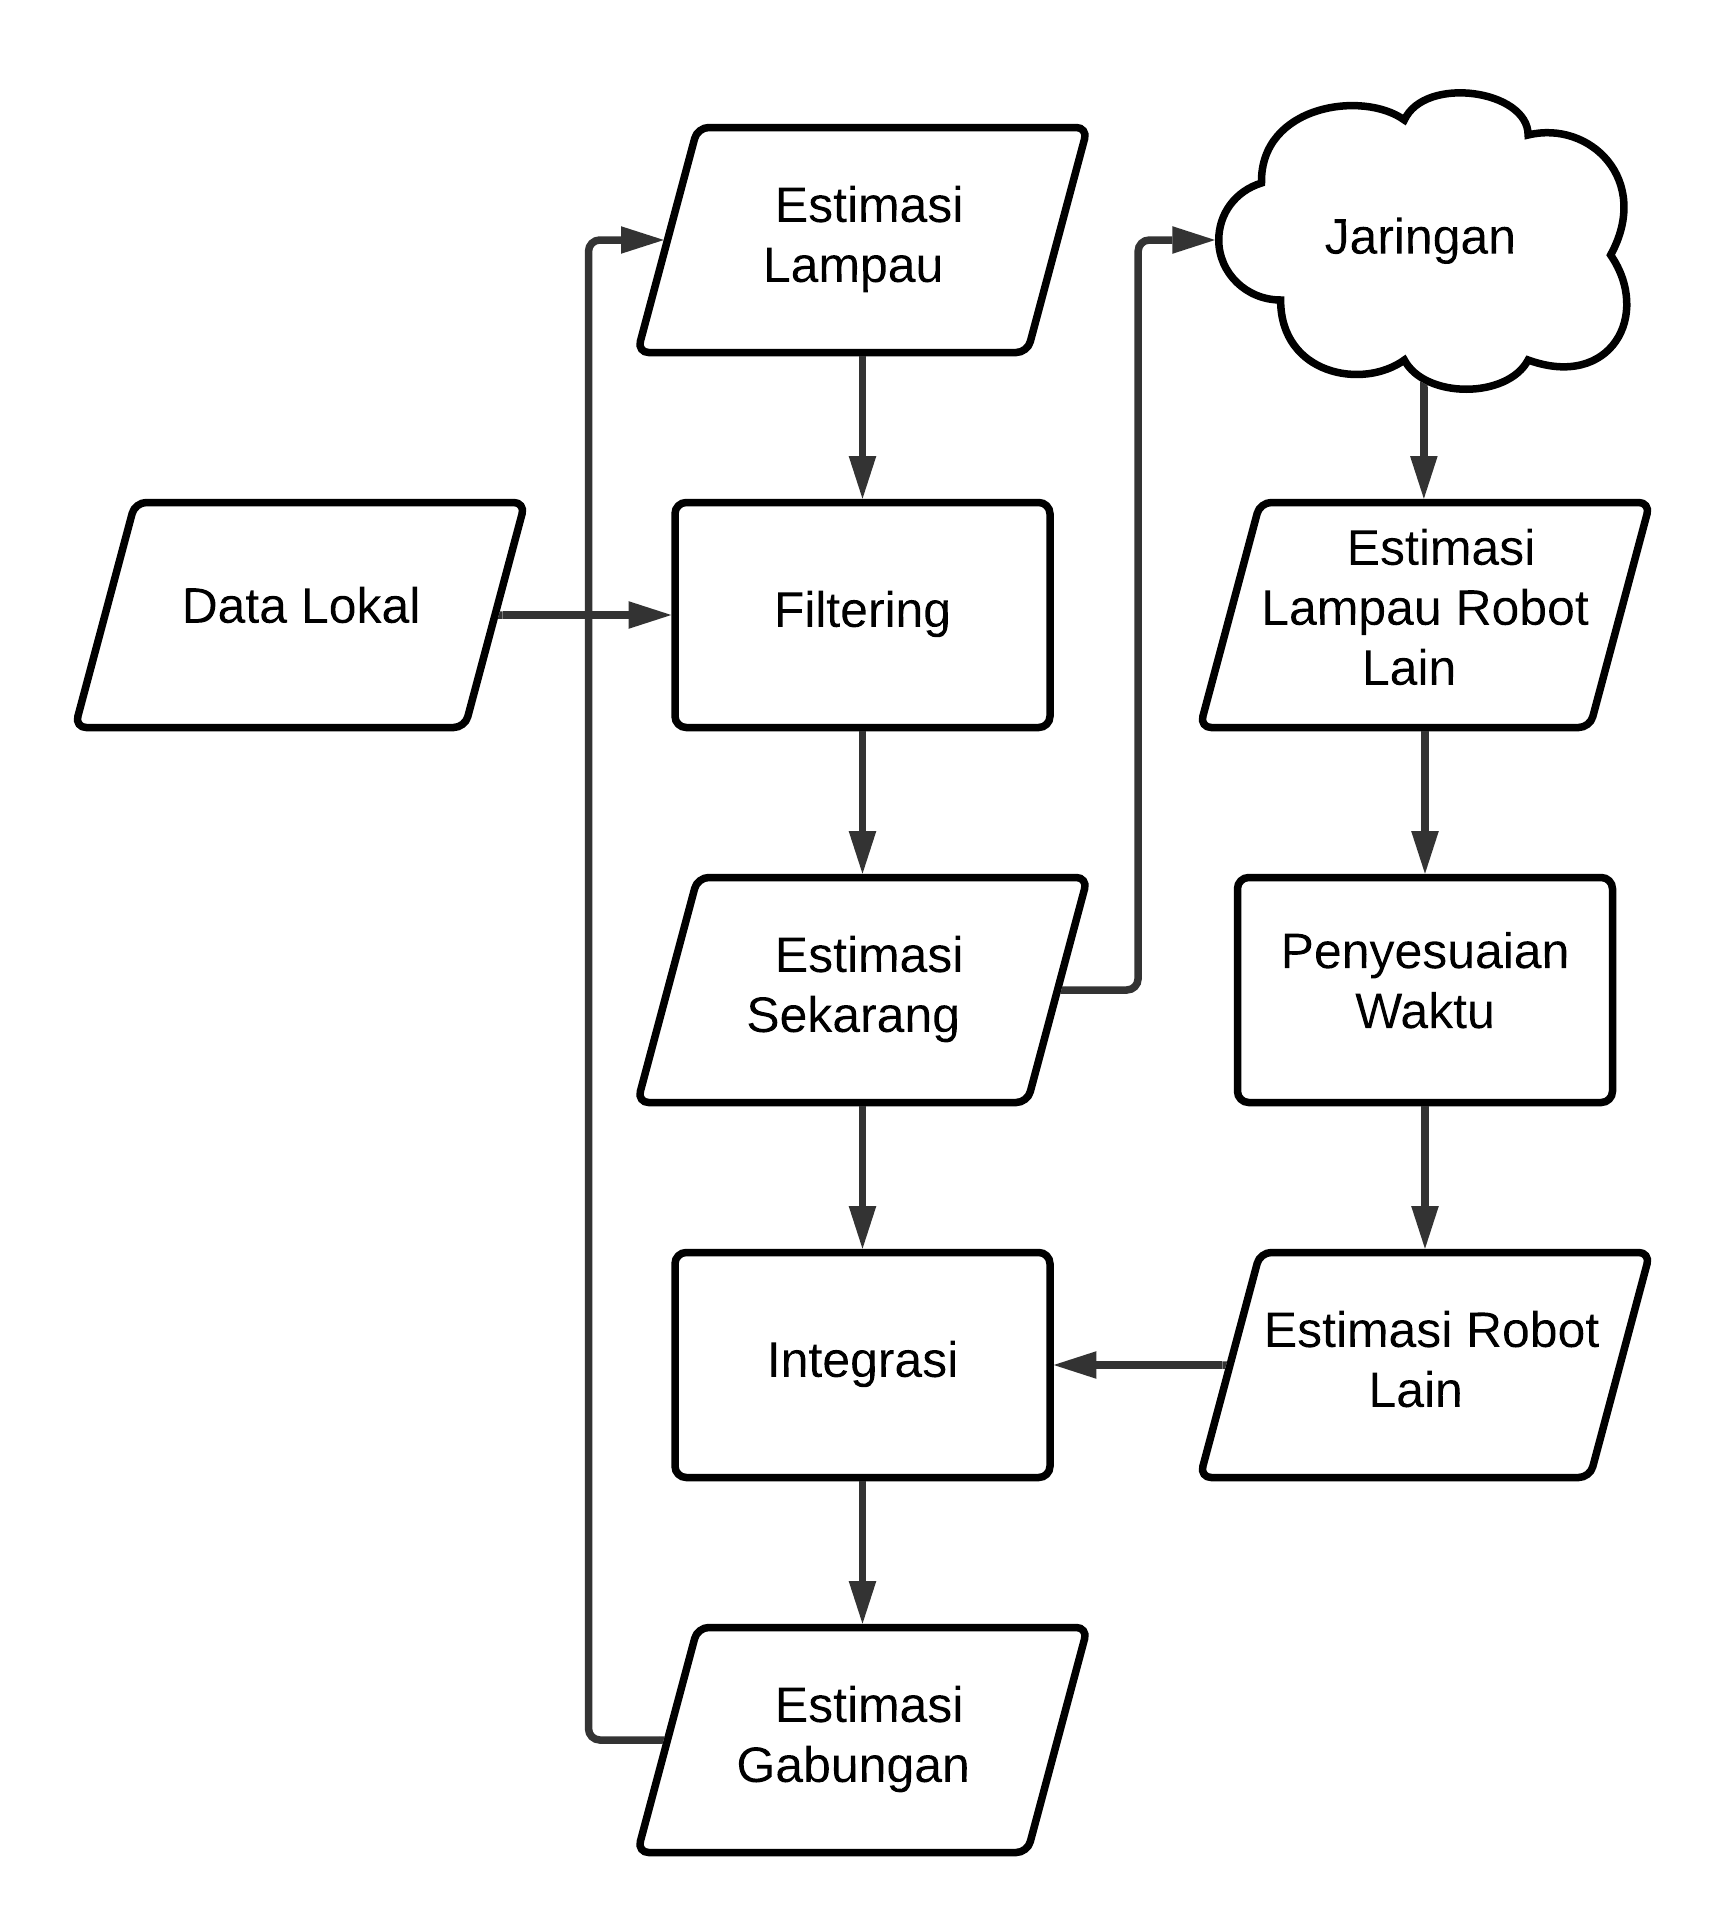
\includegraphics[width=0.8\textwidth]{resources/solution-flowchart.png}
    \caption{Diagram alir hipotesis solusi}
    \label{fig:solution-flowchart}
    \bigskip
\end{figure}

Diagram alir hipotesis solusi digambarkan di \ref{fig:solution-flowchart}. Walaupun terdapat beberapa fungsi \textit{callback} yang dapat berjalan karena \textit{event}nya masing-masing, pemanggilan fungsi \textit{callback} oleh ROS dilakukan secara sinkronis satu-persatu sehingga tidak dibutuhkan pertimbangan mengenai \textit{thread-safety} dan \textit{mutex}. Dengan periode komputasi $30$ ms, \textit{callback} periode komputasi dan \textit{callback} sensor akan dijalankan sekitar $33,3$ kali perdetik dan \textit{callback} data dari teman bergantung pada kondisi jaringan komunikasi akan dijalankan rata-rata maksimal sebanyak $66,6$ kali perdetik, sehingga kinerja algoritma tidak terlalu dituntut dalam segi konstrain waktu komputasi.

\section{Implementasi Algoritma Lokalisasi}

Algoritma estimasi gerakan robot sendiri atau algoritma lokalisasi menggunakan informasi odometri atau perpindahan, orientasi dari kompas, dan persepsi \textit{landmark} untuk mengestimasi dimana dan berapa kecepatan dari robot tersebut sekarang. Selain cara naif yang hanya mengagregasi perpindahan odometri, untuk menggunakan penapis Bayes, model pengukuran dari persepsi \textit{landmark} yang tidak linear terhadap posisi robot sesungguhnya menjadikan penapis Kalman tidak dapat digunakan untuk melakukan lokalisasi ini. Sehingga penapis partikel lebih cocok digunakan untuk menyelesaikan permasalahan ini. Khususnya algoritma \textit{AMCL} yang melakukan \textit{resampling} dianggap sebagai algoritma yang tahan terhadap kemungkinan buruknya pengukuran.

Dalam praktisnya, informasi odometri dapat digunakan baik dalam model transisi maupun model pengukuran dari penapis partikel yang digunakan, sehingga menghasilkan dua variasi dari algoritma lokalisasi yang dapat digunakan, variasi AMCL yang berbasis \textit{pose} atau variasi yang berbasis \textit{pose} dan \textit{twist}.

\subsection{Penapis Partikel Berbasis \textit{Pose}}

Pada variasi pertama, partikel yang digunakan pada penapis partikel lokalisasinya mengandung informasi tentang \textit{pose} sesungguhnya dari robot, sehingga estimasi yang dihasilkan AMCL juga berupa \textit{pose} dari robot. Sedangkan \textit{twist} dari robot diturunkan dengan mengambil perpindahan diantara hasil estimasi sekarang dengan hasil estimasi sebelumnya diturunkan terhadap selisih waktu.

Model transisi dari partikel yang ada menggunakan informasi odometri yang ada, dimana masing-masing partikel digerakan sesuai dengan perpindahan yang disampel di sekitar nilai odometri tersebut.

\begin{algorithm}
    \caption{Model pengukuran \textit{pose}}
    \label{alg:pose-measurement-model}
    \begin{algorithmic}[1]
        \Function{calc\_weight}{pose, compass, landmarks, true\_landmarks}
        \State ln\_vis\_weight = $0$
        \If{size(landmarks) != $0$}
        \State vis\_weight = $0$
        \For{landmark in landmarks}
        \State landmark\_weight = -infinity
        \For{true\_landmark in true\_landmarks}
        \State rel\_landmark = -pose + true\_landmark
        \State weight = exp(compare(landmark, rel\_landmark))
        \State landmark\_weight = max(landmark\_weight, weight)
        \EndFor
        \State vis\_weight += landmark\_weight
        \EndFor
        \State ln\_vis\_weight = log(vis\_weight / size(landmarks))
        \EndIf
        \State ln\_ort\_weight = compare(pose.orientation, compass)
        \State return exp($\alpha \times$ ln\_vis\_weight + $\beta \times$ ln\_ort\_weight)
        \EndFunction
    \end{algorithmic}
\end{algorithm}

Model pengukuran menggunakan informasi \textit{landmark} dimana untuk masing-masing partikel, semua pengukuran \textit{landmark} yang ada dibandingkan dengan semua posisi absolut \textit{landmark} yang sebenarnya untuk diambil peluang terukurnya pengukuran tersebut berdasarkan profil \textit{error} normal independen. Diambil peluang pengukuran terbesar untuk masing-masing pengukuran yang berikutnya dirata-ratakan untuk masing-masing partikel. Selain itu, pengukuran dari kompas berdasarkan distribusi \textit{error} normal dari orientasi sebenarnya juga digunakan. Kedua peluang dari pengukuran \textit{landmark} dan dari pengukuran kompas diintegrasi dengan melakukan perkalian setelah masing-masing peluang dipangkatkan oleh suatu \textit{weight} faktor pengukuran. Fungsi yang digunakan digambarkan pada \ref{alg:pose-measurement-model} dimana fungsi compare menghasilkan logaritma natural dari peluang dilakukannya pengukuran, yang berdasarkan persamaan distribusi normal hanyalah bernilai $-0,5$ dikali jarak kuadrat dibagi dengan variansi.

Hasil prediksi dari suatu iterasi estimasi adalah rata-rata dari partikel yang ada, dimana posisi dirata-ratakan sebagai vektor dan orientasi dirata-ratakan dengan mengambil arah dari rata-rata vektor unit dengan arah orientasi masing-masing partikel. Sedangkan \textit{resampling} dilakukan dengan mengambil \textit{pose} di sekitar rata-rata partikel tersebut ditambah \textit{error} dengan distribusi normal.

\subsection{Penapis Partikel Berbasis \textit{Pose} dan \textit{Twist}}

Pada variasi kedua, partikel yang digunakan mengandung informasi tentang \textit{pose} dan juga \textit{twist} dari robot, sehingga pada variasi ini tidak perlu diturunkan lagi \textit{twist} dari robot secara terpisah karena sudah menjadi bagian dari hasil estimasi penapis.

Pada variasi ini nilai odometri tidak digunakan pada model transisi. Model transisi mengandalkan pada \textit{twist} yang sudah dimiliki masing-masing partikel, dimana \textit{twist} tersebut ditambahkan dengan \textit{error} normal untuk membangkitkan \textit{twist} baru dan \textit{pose} baru dibangkitkan dengan meng\textit{update} \textit{pose} lama menggunakan \textit{twist} yang baru dibangkitkan.

Model pengukuran variasi ini mirip dengan model pada variasi pertama dalam caranya menggunakan pengukuran \textit{landmark} dan kompas. Di variasi ini, odometri juga digunakan pada model pengukuran dengan membandingkannya dengan perpindahan sebenarnya yang dapat didapatkan dari mengintegrasi \textit{twist} partikel dengan selisih waktu.

Rata-rata partikel diambil dengan cara yang sama untuk \textit{pose} dari partikel dan analog untuk mendapatkan rata-rata dari \textit{twist} partikel. \textit{Resampling} juga dilakukan di sekitar \textit{pose} dan \textit{twist} partikel rata-rata dengan penambahan \textit{error}.

\section{Estimasi Gerakan Bola}

Estimasi gerakan bola berdasarkan data persepsi bola yang didapat dari sensor sendiri atau teman lebih leluasa dibandingkan dengan lokalisasi. Hal ini dikarenakan bacaan posisi bola bersifat linear terhadap posisi bola sesungguhnya ditambah suatu \textit{error} seperti yang ada pada asumsi penapis Kalman. Oleh karena itu, walaupun profil \textit{error} sesungguhnya dari bacaan posisi bola tidak \textit{uniform} untuk semua posisi sesungguhnya, dapat dimodelkan \textit{error} normal \textit{uniform} untuk dapat menggunakan penapis Kalman dalam melakukan estimasi gerakan bola. Karena bacaan posisi bola yang dilihat bersifat relatif, maka estimasi gerakan bola mengandalkan estimasi gerakan robot yang melakukan persepsi untuk mengubah bacaan posisi bola yang relatif ke ruang referensi absolut.

\subsection{Estimasi dengan Penapis Kalman}

Penapis Kalman memodelkan distribusi gerakan bola sebagai distribusi normal multivariat dengan vektor rata-rata $\mu$ empat dimensi yang merepresentasikan komponen posisi bola pada sumbu x, kecepatan pada sumbu x, posisi pada sumbu y, dan kecepatan pada sumbu y, juga matriks kovarian $4 \times 4$ dengan urutan komponen yang sama.

Karena informasi bola hanya berupa pengukuran, tidak ada variable transisi yang digunakan dalam estimasi gerakan bola. Sehingga persamaan transisi yang digunakan hanyalah
\begin{align}
    x_t = A_t x_{t-1} + \epsilon_t \,
\end{align}
dimana $A_t$ adalah matriks $4 \times 4$ \textit{update} keadaan dimana posisi baru ditambahkan dengan kecepatan dikalikan selisih waktu, sedangkan $\epsilon_t$ adalah vektor acak \textit{error} empat dimensi. Variansi dari komponen \textit{error} kecepatan adalah konstanta dikali selisih waktu. Karena perubahan posisi adalah perubahan kecepatan dikali selisih waktu, maka didapatkan variansi komponen \textit{error} posisi adalah konstanta dikali selisih waktu pangkat tiga dan kovarian antara komponen \textit{error} posisi dan kecepatan adalah konstanta dikali selisih waktu kuadrat.

Pada persamaan pengukuran $z_t = C_t x_t + \delta_t$, $z_t$ adalah vektor dua dimensi berisi pengukuran posisi absolut bola pada sumbu x dan y. $C_t$ adalah matriks pengukuran berdimensi $2 \times 4$ yang bernilai $1$ di komponen posisi yang terkait dan $0$ di sisanya. Walaupun distribusi \textit{error} pengukuran bola tergantung dari posisi robot yang melihat dan jarak bola dengan robot, karena dibutuhkan suatu vektor acak $\delta_t$ yang sama atau \textit{uniform} untuk semua posisi, maka digeneralisasi $\delta_t$ sebagai vektor dua dimensi dengan matriks kovariansi $Q_t$ merupakan matriks identitas dikali suatu konstanta.

\subsection{Estimasi dengan Penapis Partikel}

Estimasi gerakan bola dengan penapis partikel mirip dengan algoritma lokalisasi variansi dua, dimana sampel berisi posisi dan kecepatan dari bola dan tidak ada kalkulasi terpisah untuk menentukan kecepatan dari bola. Tidak ada variabel transisi yang dapat digunakan, jadi model transisi hanyalah membangkitkan kecepatan baru di sekitar kecepatan partikel dan meng\textit{update} posisi berdasarkan kecepatan baru dan selisih waktu seperti pada lokalisasi variansi dua.

Model pengukuran menggunakan persamaan yang sama dengan pengukuran menggunakan \textit{landmark}, dimana posisi robot yang melakukan persepsi mengandalkan hasil lokalisasi untuk menghasilkan posisi relatif bola referensi untuk dibandingkan dengan posisi relatif bola yang dilihat.

\section{Integrasi Data Bola Terlambat}

Cara integrasi data bola dari teman yang paling dasar adalah dengan mengintegrasinya ke dalam penapis bola yang digunakan, sama seperti dengan pemrosesan data sensor, apabila dilihat bahwa \textit{timestamp} dari data tersebut lebih baru daripada data terakhir yang sudah diproses. Kekurangan dari metode ini adalah apabila robot sendiri dan satu atau lebih teman melihat bola pada saat yang sama, informasi yang didapat dari teman tersebut tidak akan pernah digunakan karena data sensor dari robot sendiri hampir pasti sampai lebih cepat dibandingkan dengan data dari teman yang ditambahkan dengan latensi komunikasi. Salah satu cara untuk menangani hal ini adalah dengan menggunakan modifikasi penapis untuk \textit{out of order measurement} atau (\textit{OOSM}).

\subsection{Estimasi dengan OOSM-PF}

Karena tidak ada konstrain waktu ataupun memori yang signifikan, penanganan data terlambat dapat dilakukan menggunakan penyimpanan dan penyisipan data pengukuran. Pada penapis partikel OOSM-PF, untuk batas jumlah yang telah ditentukan sebelumnya, beberapa data pengukuran dan \textit{state} estimasi yang terakhir disimpan secara terurut berdasarkan \textit{timestamp} datanya. Sistem penyimpanan dapat menggunakan tipe data seperti \textit{map} terurut yang menyimpan datanya secara terurut berdasarkan \textit{key}nya yang diimplementasi di atas tipe data seperti \textit{red-black tree}. Dalam kasus penapis partikel, \textit{state} yang dimaksud adalah kumpulan partikel dalam penapis dan nilai dari $w_fast$ dan $w_slow$.

Apabila ditemui data terlambat yang lebih lama dari data terlama yang disimpan, maka data tersebut dibuang dan dikembalikan hasil estimasi terakhir. Apabila data tersebut lebih baru, cari data paling baru yang disimpan yang lebih lama dari data terlambat tersebut. Lalu simpan data terlambat tersebut dengan menghitung \textit{state}nya menggunakan algoritma penapis partikel biasa menggunakan \textit{state} sebelumnya dari data paling baru tersebut. \textit{Update} juga semua \textit{state} dari data yang disimpan yang ada setelah data yang baru dimasukan, dan buang data terlama yang disimpan apabila sudah melebihi jumlah maksimal data yang disimpan.

Kompleksitas waktu dan ruang dari algoritma ini berkembang secara linear terhadap batas jumlah data yang disimpan. Akan tetapi karena data yang sudah melewati beberapa periode komputasi semakin lama tidak relevan, maka batas jumlah ini tidak perlu diatur dengan besar.

\subsection{Estimasi OOSM-PF dengan Data Bola Opsional}

Karena kegagalan persepsi bola oleh robot juga sebenarnya memberikan informasi mengenai posisi bola dimana kegagalan posisi bola yang sebenarnya kemungkinan berada di luar radius penglihatan robot, maka dapat dibuat variasi dari penapis partikel bola yang dapat menerima data bola secara opsional. Pemanggilan penapis partikel tanpa adanya informasi bola yang menandakan bahwa kemungkinan bola berada di luar radius penglihatan mengakibatkan algoritma model pengukuran meninggikan \textit{weight} partikel yang berada di luar radius penglihatan dan mengurangi \textit{weight} partikel yang berada di dalam radius penglihatan.

Algoritma ini hanya mungkin berfungsi dengan baik menggunakan modifikasi data \textit{OOSM}. Ini disebabkan karena jika digunakan cara integrasi dasar yang hanya mempertimbangkan \textit{timestamp}, maka robot hanya akan mempertimbangkan data dari sensor sendiri saja walaupun bola tidak terlihat, karena informasi dari teman yang hampir pasti terlambat walaupun mungkin teman tersebut melihat posisi bola sehingga informasinya lebih berguna dibandingkan informasi robot sendiri yang tidak melihat bola.

\subsection{Estimasi dengan OOSM-KF}

OOSM-KF adalah algoritma seperti OOSM-PF akan tetapi menggunakan algoritma penapis Kalman sebagai dasarnya. Perbedaan dari algoritma ini adalah \textit{state} yang disimpan hanyalah berupa representasi distribusi normal multivariat berupa vektor rata-rata dan matriks kovariansi, sehingga kompleksitas waktu dan ruangnya setaraf lebih efisien dibandingkan OOSM-PF.

\subsection{Estimasi OOSM-KF dengan Data Bola Kombinasi}

Salah satu cara konvensional untuk menggabungkan data posisi bola dari banyak robot adalah dengan merata-ratakan data tersebut. Variansi OOSM-KF dengan data bola kombinasi adalah variansi OOSM-KF bola dimana apabila diterima dua atau lebih data dengan \textit{timestamp} yang sama dari beberapa robot, maka data tersebut tidak akan diproses satu-persatu, melainkan dengan dirata-ratakan dan diproses dengan sekaligus. Variansi ini menggunakan penapis Kalman karena rata-rata posisi absolut bola yang digunakan dengan kemungkinan bola dilihat lebih dari satu robot, sehingga penapis partikel yang membutuhkan satu robot yang melihat bola untuk menentukan profil \textit{error} dari bacaan tidak dapat digunakan.

\section{Koreksi Gerakan Robot Teman dengan Persepsi \textit{Vision}}

Walaupun hasil persepsi robot teman dari suatu robot memiliki \textit{error} yang cukup tinggi jika dibandingkan dengan hasil lokalisasi oleh teman tersebut menggunakan odometri, kompas, dan beberapa persepsi \textit{landmark}, hasil persepsi tersebut lebih tersedia karena bersumber dari sensor sendiri jika dibandingkan dengan hasil lokalisasi teman yang harus melalui latensi jaringan, terutama apabila kondisi jaringan yang sedang buruk. Oleh karena itu, persepsi robot teman menjadi informasi yang berguna karena dapat digunakan untuk mengoreksi estimasi robot sendiri mengenai gerakan robot teman.

Karena informasi hasil lokalisasi teman tersebut tetap lebih berharga dibandingkan persepsi melalui \textit{vision}, digunakan OOSM-PF untuk mencampurkan data dari teman yang terlambat dengan persepsi \textit{vision} yang selalu ada. Algoritma penapis partikel yang digunakan menyediakan dua jenis antarmuka fungsi estimasi, yaitu fungsi yang menerima data dari teman berupa \textit{pose} dan \textit{twist} secara absolut dan fungsi yang menerima data dari sensor berupa posisi relatif teman tersebut. Walaupun model transisinya sama, model pengukuran dari data teman membandingkan jarak nilai \textit{pose} dan \textit{twist} estimasi dan partikel, sedangkan model pengukuran dari data sensor sama seperti penapis partikel bola yang membandingkan posisi relatif robot teman referensi dengan yang dilihat.

Sensor \textit{vision} yang tidak dapat membedakan teman yang mana yang sedang dilihat mengakibatkan kebutuhan suatu algoritma yang dapat menentukan siapa robot teman yang dilihat berdasarkan posisinya. Dibuat matriks \textit{cost} yang menyimpan \textit{cost} dalam mencocokan suatu persepsi teman dengan identitas robot teman tersebut. \textit{Cost} berupa jarak kuadrat dari posisi absolut persepsi robot teman tersebut dengan estimasi posisi sesungguhnya suatu identitas robot teman berdasarkan estimasi yang sudah disesuaikan waktunya. Dari sini, masalah penyeleksian identitas teman dapat diselesaikan dengan algoritma seperti \textit{Hungarian algorithm}, tetapi untuk kasus kemungkinan robot teman yang sedikit, dapat langsung di\textit{brute-force} untuk menentukan penyeleksian dengan jumlah \textit{cost} minimum.
